\subsection{ALOCAÇÃO DE MATÉRIAS}

Durante os incrementos anterioriores, o otimizador gerava grades horárias que continham apenas os nomes dos professores alocados para aula. Em outras palavras, as grades eram matrizes nas quais as linhas eram os horários disponíveis, as colunas eram as salas e cada posição na matriz representava qual professor deveria ministrar a aula naquele horário.

A alocação dos professores é muito importante para a resolução do problema, pois apresenta a maior parte das retrições e dificuldades relacionadas, como os conflitos, por exemplo. Entretando, em termos de completude, as grades horárias devem ter também a alocação de matérias em cada horário de aula, visto que cada professor pode ministrar aulas de mais de uma matéria. As alterações necessárias para possibilitar isso foram:

\begin{enumerate}
	\item Alterar a modelagem do banco de dados para comportar informações relacionadas às matérias;
	\item Alterar telas da interface web para que fosse possível configurar as matérias;
	\item Alterar rotas do servidor para persistir as matérias;
	\item Alterar código do otimizador para produzir grades horárias com matérias
\end{enumerate}

\subsubsection{Alteração no banco de dados}
Para armazenar informações relacionadas às matérias, a modelagem do banco de dados foi alterada com a criação de uma tabela para armazenar as matérias, e a adição de uma coluna à tabela ``horario'' aula para que seja possível especificar matérias alocadas nas grades horárias. 
Com estas alterações, a modelagem do banco de dados passa a ser representada pela figura \ref{fig:modelagemMateiras}.

\begin{figure}[!htb]
	\centering
	\caption{Modelo Entidade-Relacionamento com Matérias}
	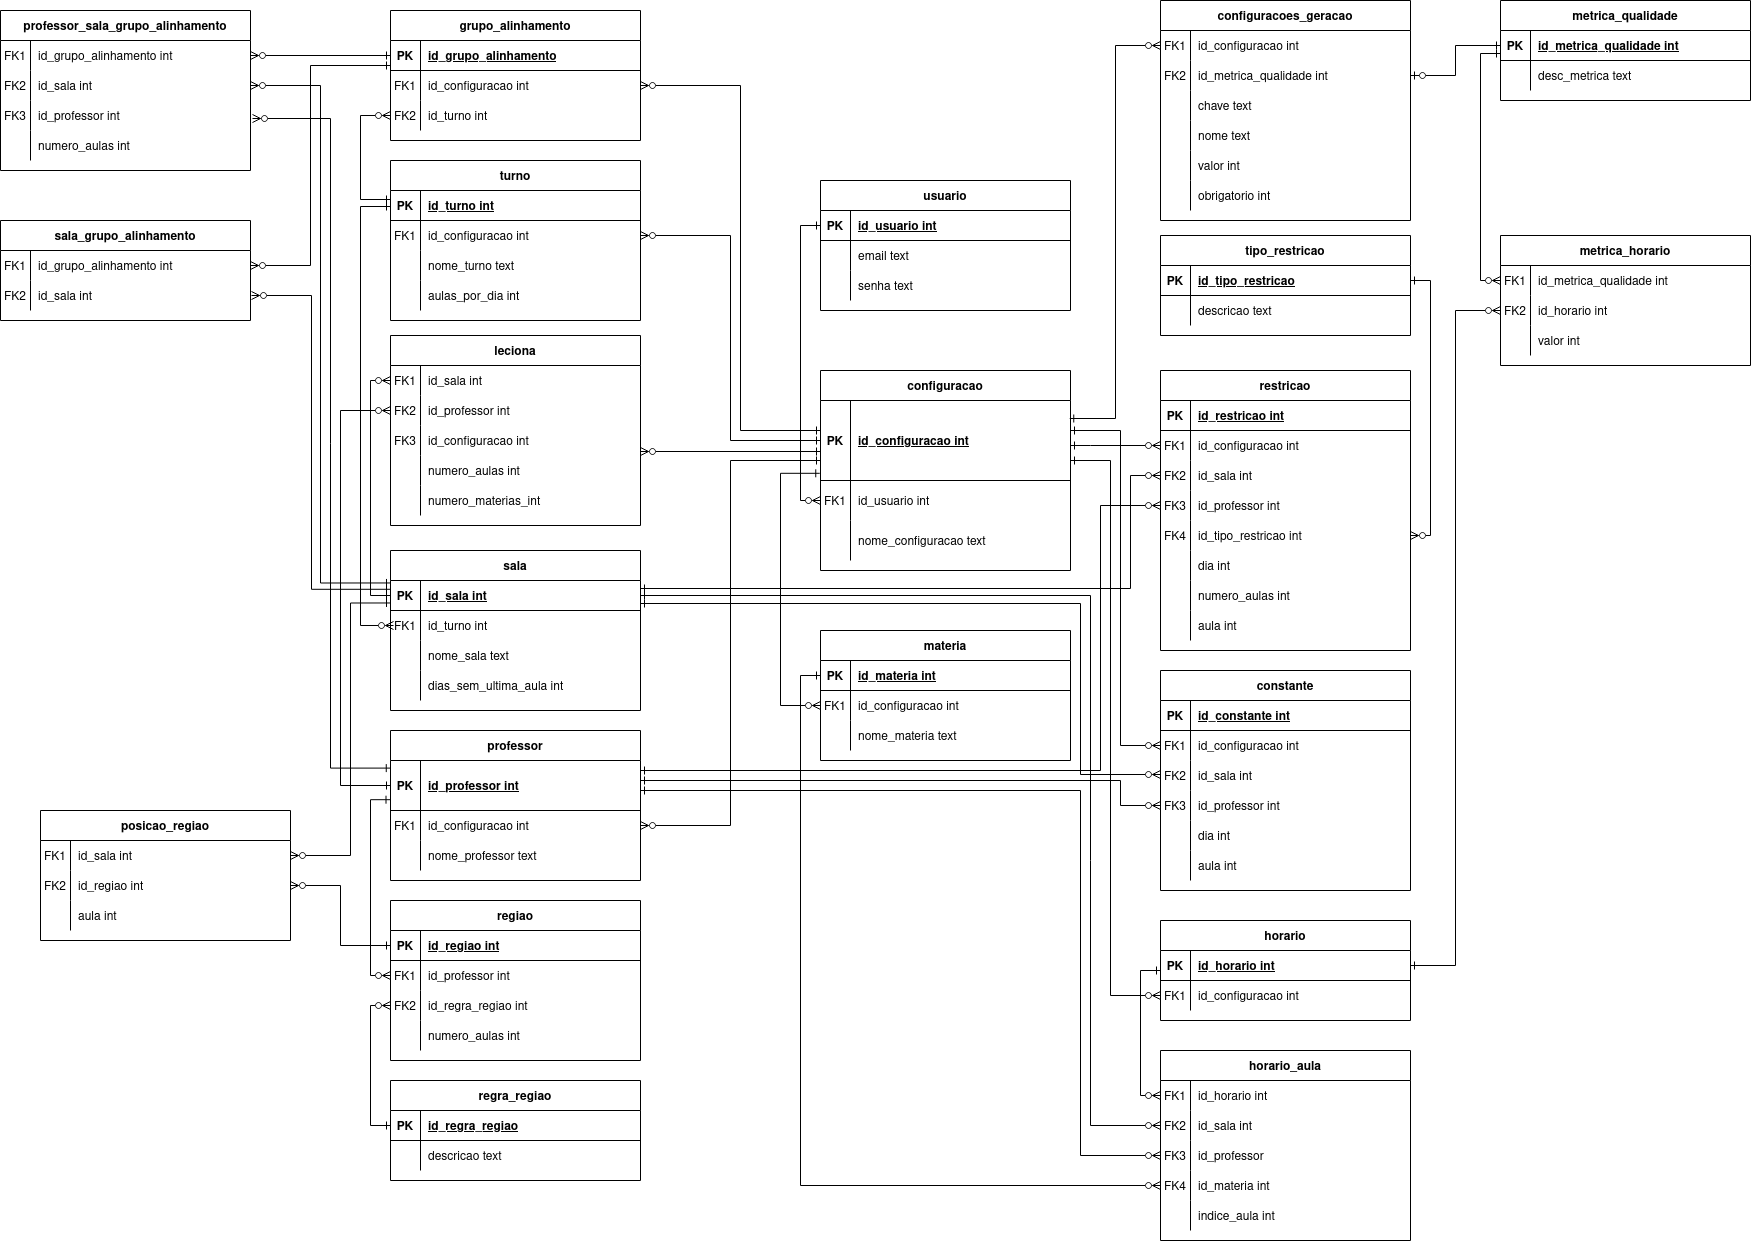
\includegraphics[width=1\textwidth]{./dados/figuras/ER_horario_INCREMENTO6}
	\fonte{Autor}
	\label{fig:modelagemMateiras}
\end{figure}
\pagebreak

\subsubsection{Alteração de telas}
Com a adição do conceito das matérias ao sistema, algumas telas da interface precisaram ser modificadas. A primeira destas, foi a tela inicial da configuração, ou seja, a tela de "Estrutura da Escola", cuja alteração pode ser vista na figura \ref{fig:estruturaAtualizada} consistiu na adição de uma seção para cadastro e visualização de matérias, semelhante ao componente de cadastro de professores.

\begin{figure}[!htb]
	\centering
	\caption{Estrutura da Escola com Matérias}
	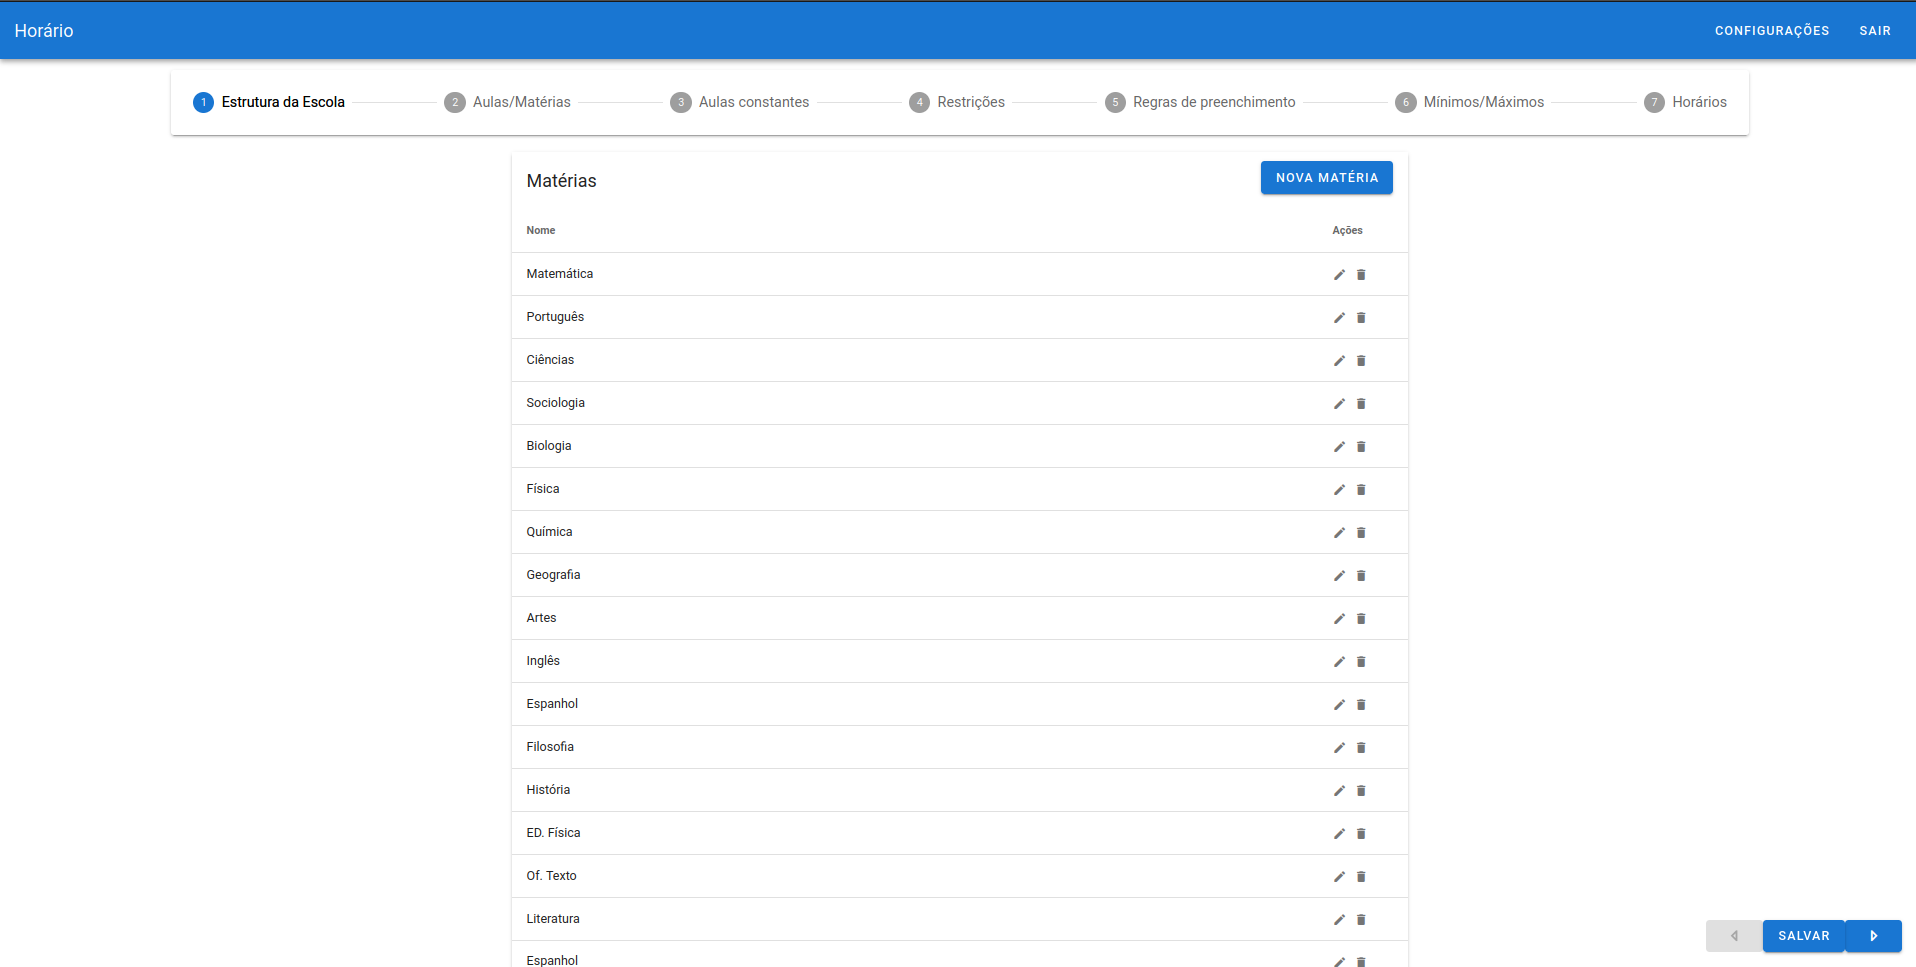
\includegraphics[width=0.65\textwidth]{./dados/figuras/alteracaoEstrutura}
	\fonte{Autor}
	\label{fig:estruturaAtualizada}
\end{figure}
\pagebreak

Além da tela de estrutura, a segunda aba da configuração ("Aulas/Matérias") foi alterada para que fosse possível vincular matérias aos professores, e configurar a quantidade de aulas de cada matéria deve ser ministrada semanalmente, conforme a figura \ref{fig:alteracaoAulas}.

\begin{figure}[!htb]
	\centering
	\caption{Tela de configuração de quantidades de aulas por matéria}
	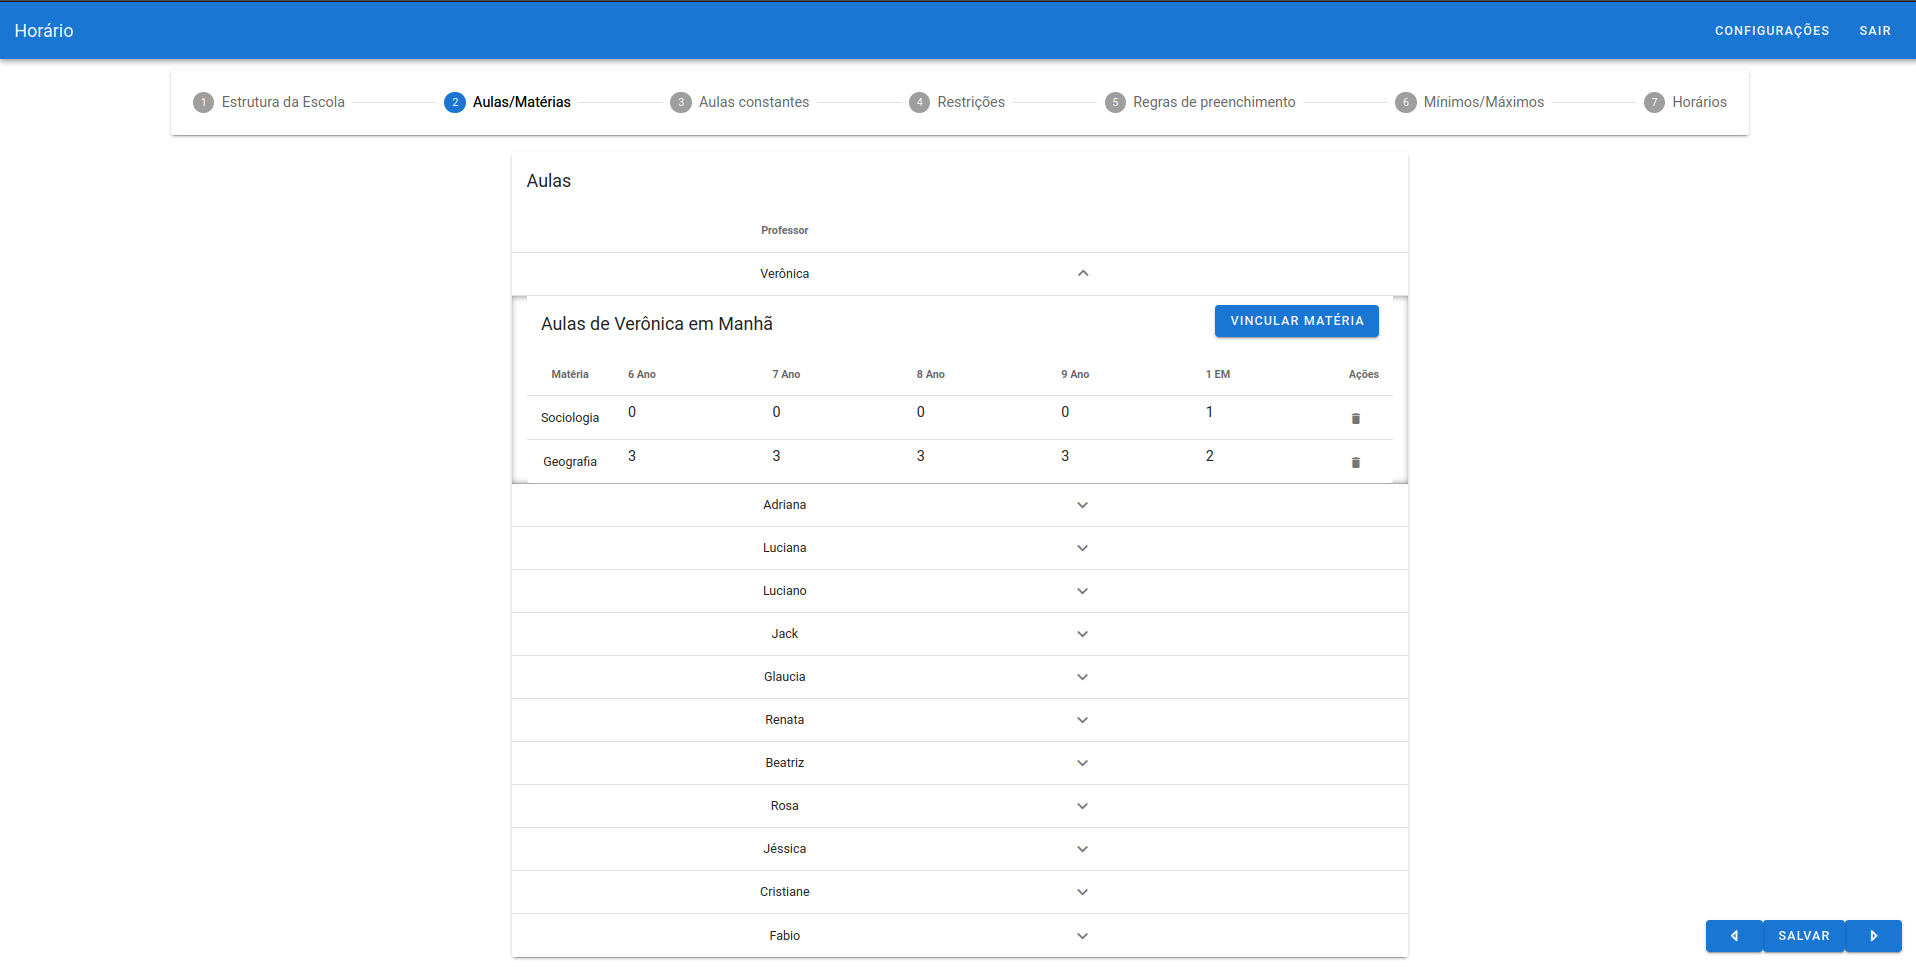
\includegraphics[width=0.65\textwidth]{./dados/figuras/alteracaoAulas}
	\fonte{Autor}
	\label{fig:alteracaoAulas}
\end{figure}

Por fim, na tela final da configuração, responsável por exibir as grades horárias geradas, foi necessário alterar o componente da grade para incluir, além dos nomes dos professores, os nomes das matérias alocadas para cada horário, como pode ser visto na figura \ref{fig:alteracaoHorario}.

\begin{figure}[!htb]
	\centering
	\caption{Visualização de grade horária com matérias}
	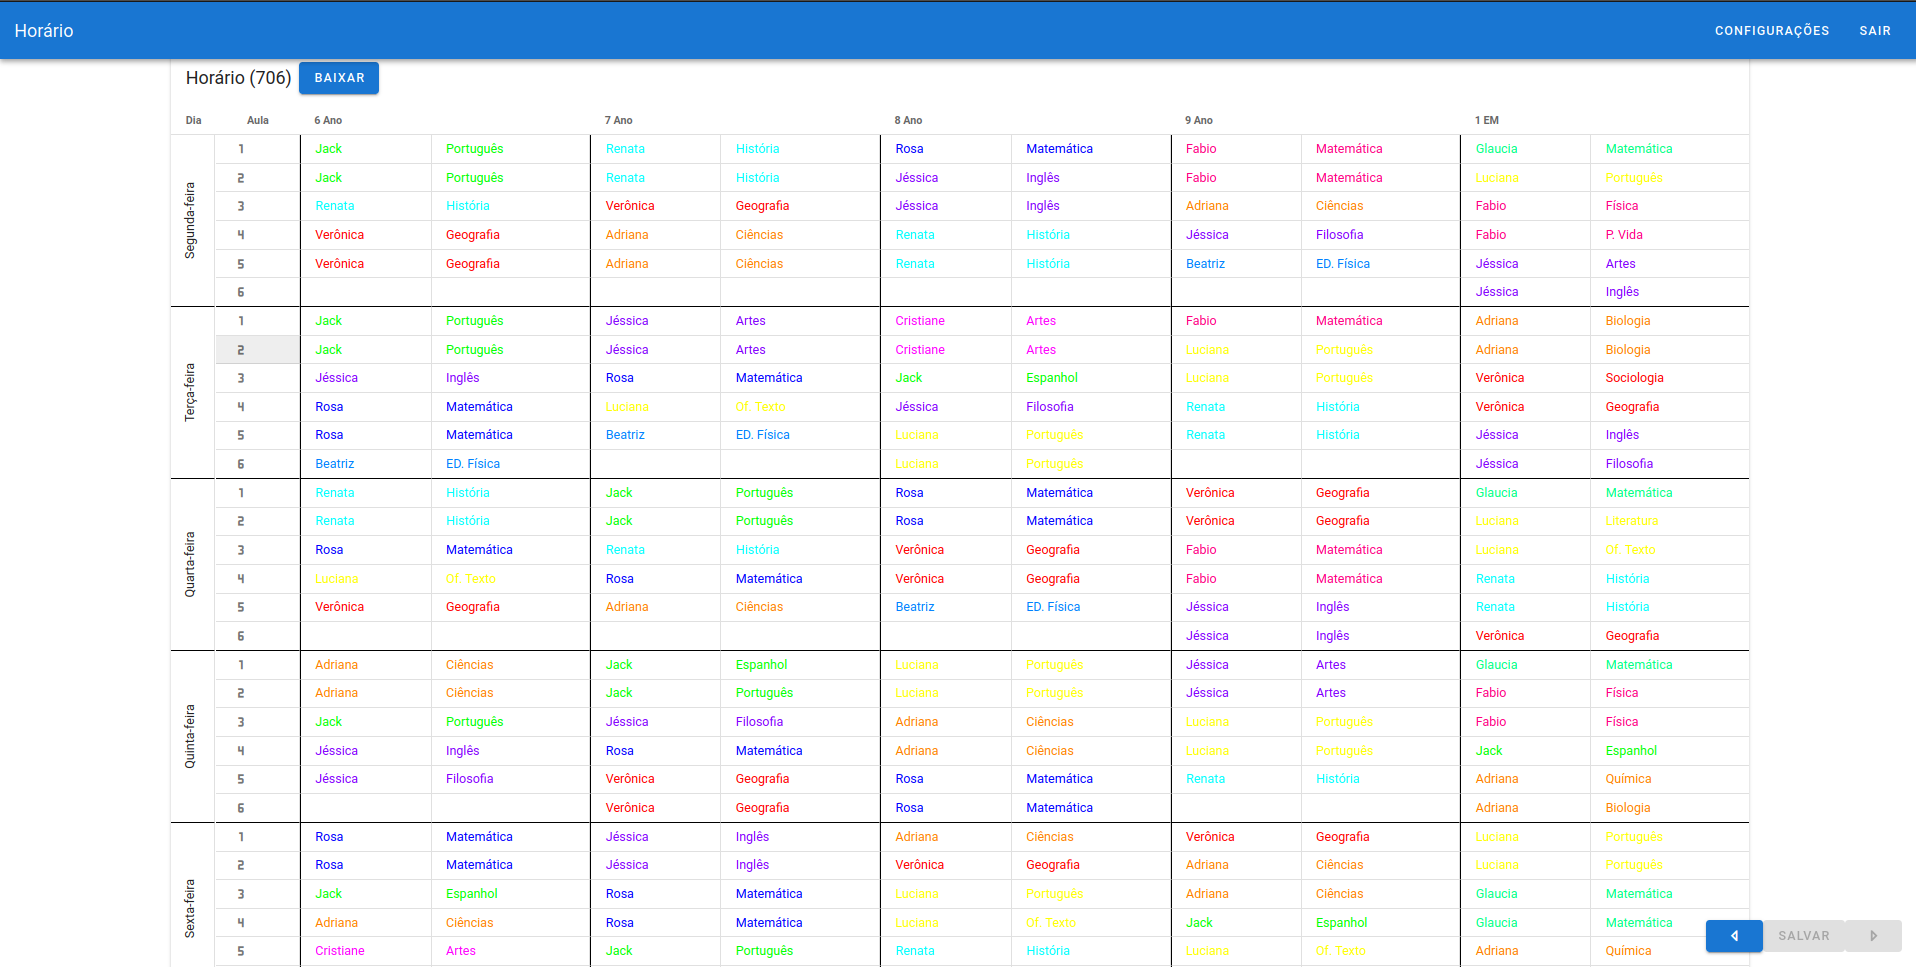
\includegraphics[width=0.65\textwidth]{./dados/figuras/alteracaoHorarios}
	\fonte{Autor}
	\label{fig:alteracaoHorario}
\end{figure}

\subsubsection{Alteração de métodos no servidor}
A adição das matérias também envolveu algumas alterações no servidor. As rotas alteradas para acomodar a melhoria foram rotas de armazenamento e consulta da estrutura da escola, aulas e grades horárias.

Evidentemente, foi necessário criar rotas também para o gerenciamento de matérias, e as demais rotas do sistema precisaram ter suas funções de tratamento modificadas para interagir corretamente com esta nova tabela.

\subsubsection{Matérias no otimizador}
Após as alterações na interface, servidor e banco de dados, o sistema estava pronto para lidar com as informações relacionadas às matérias, faltando apenas a incorporação destas na geração de grades horárias por parte do otimizador. 

Para realizar isso, o otimizador foi alterado para alocar também matérias na grade horária, de forma que enquanto antes a grade horária armazenava em cada posição um professor que foi alocado para aquele horário, agora passa a armazenar uma dupla de professor e matéria alocados. Durante os passos de otimização, estas duplas seão permutadas, garantindo assim que cada matéria sempre corresponde a um professor compatível. Com estas alterações, o algoritmo \ref{alg:otimizadorCompleto} passa a representar o otimizador.


\begin{algorithm}
	\caption{Otimizador com alocação de matérias}
	\label{alg:otimizadorCompleto}
	\KwIn{Lista de professores $LP$, lista de turmas $LT$, matriz de aulas e matérias por professor por turma $MA$, temperatura inicial $TI$, Taxa de resfriamento $TR$}
	\KwOut{Grade horária de matérias e professores otimizada}
	$temperatura \leftarrow TI$\\
	$grade \leftarrow$ CriaGradeInicial$(LP, LT, MA)$\\
	$iteracoesSemAlteracao \leftarrow 0$\\
	$solucoes \leftarrow$ lista vazia\\
	\While {condição de parada não atingida} {
		$deltaTotal \leftarrow 0$\\
		\For {$passo = 0$ até $numeroPassos$} {
			$turma \leftarrow grade.EscolheTurmaAleatoria()$\\
			$duplas \leftarrow grade.EscolheDuplasAleatoriasValidas(turma)$\\
			$delta \leftarrow grade.CalculaDelta(turma, duplas)$\\
			$probabilidade \leftarrow e^{-delta/temperatura}$\\
			$valorAceite \leftarrow ValorAleatorioEntre(0, 1)$\\
			\If {$delta < 0$ ou $probabilidade \ge valorAceite$} {
				$grade.PermutaDuplas(sala, duplas)$\\
				$deltaTotal \leftarrow deltaTotal + delta$\\
				\If {grade não existe na lista de soluções} {
					insere grade na lista de soluções\\
					limita lista de soluções às 100 melhores grades\\
				}
			}
		}
		\eIf {$delta = 0$} {
			$iteracoesSemAlteracao \leftarrow iteracoesSemAlteracao + 1$\\
		}{
			$iteracoesSemAlteracao \leftarrow 0$\\
		}
		\If {$iteracoesSemAlteracao \ge 15$} {
			salvaGradesRelevantes()\\
			apaga lista de soluções\\
			$temperatura \leftarrow TI$\\
			$iteracoesSemAlteracao \leftarrow 0$\\
		}
		$temperatura \leftarrow temperatura * TR$
	}
\end{algorithm}
\pagebreak